\section{Introduction}
% combine first two §?
In contemporary radiation therapy, photon intensity modulated radiation therapy (IMRT) is a pivotal technique to attain precise and conformal dose distributions within target volumes \cite{xu_comparison_2017}.
This achievement owes its realization to the advent of the multileaf collimator (MLC) \cite{galvin_characterization_1993}.

Radiation therapy is now a reliable treatment for oncology \cite{valentini_survival_2009}.
Despite this consensus, the way to deliver radiotherapy for its best result remains very dependent upon doctors.
Moreover, there appears to be a large variability across physicians and centres, but in terms of 3D structures contouring and irradiation, constrains priorities \cite{variability_2021}.

To achieve the best treatment, doctors must solve a complex inverse mathematical optimization problem with multiple trade-offs \cite{oelfke_inverse_2001} \cite{webb_physical_2003}.
%However, a lack of standardization ...
A lack of standardized prioritization of constraints makes the optimization a real challenge.
The standard procedure nowadays is to guide computer optimization manually: dosimetrists manually update the settings of an optimizing software so-called Treatment Planning System (TPS) \cite{planification_website}.

There have been many tries to create a metric that quantifies the quality of a treatment plan, such as Normal tissue complication probabilities (NTCP), Target coverage, Conformity index, and Heterogeneity index, among others/to name a few \cite{lyman_normal_1992} \cite{li_input_2022}.\label{metrics}
However, they have yet to satisfy all radio-oncologists, and the only reliable way to assess a doctor's plan is to assess out the dose-volume histograms (DVHs) themselves.

As a result, Pareto surface exploration is unsuitable due to the lack of impartial quantitative measurement for a particular plan \cite{huang_pareto_2021}.
Other meta-optimization techniques are similarly bounded for the same reason \cite{wu_optimization_2001} \cite{xing_optimization_1999}.
An extra challenge to attend for those is the fact that not all cases have the same "difficulty."
Hence, for an "easy" case, doctors will require an excellent dose (in terms of the metrics mentioned above), while they can be more permissive for "harder" cases.
This makes the acceptability of a plan hard to define in general.

Reinforcement learning is a machine learning paradigm that trains agents to make sequential decisions in dynamic environments \cite{brooks_what_2021}.
Through trial and error guided by rewards or penalties, agents learn to optimize their actions to achieve long-term objectives.
The decisions taken by dosimetrists when optimizing treatment can be formalized as a reinforcement learning problem.
Moreover, dosimetrists can guide the TPS towards an acceptable plan but usually struggle to explain their decision while interacting with the TPS.
The difficulty in explaining why certain decisions are taken suggests using deep reinforcement learning over expert-based methods.
This setup is similar to image recognition, where one can say a picture represents a car or a boat but struggles to explain why.

We sought to leverage deep learning to learn the actions a dosimetrist takes when optimizing a dose using a treatment planning system.
The study’s primary hypothesis was that all the information needed to decide what weights should be changed in the objective function used by the optimizer relies on the Dose Volume Histograms (DVHs).
This assumption is supported by the fact that dosimetrists almost solely use those DVHs plots.
We trained an agent that takes as an input the DVHs of the current optimized dose, and predicts the evaluation of possible weights changes.

\section{Materials and Methods}
We introduce a new paradigm in reinforcement learning (RL) based on evaluating states rather than the reward.

\subsection{Reinforcement Learning Reward}

\begin{figure*}
	\centering
	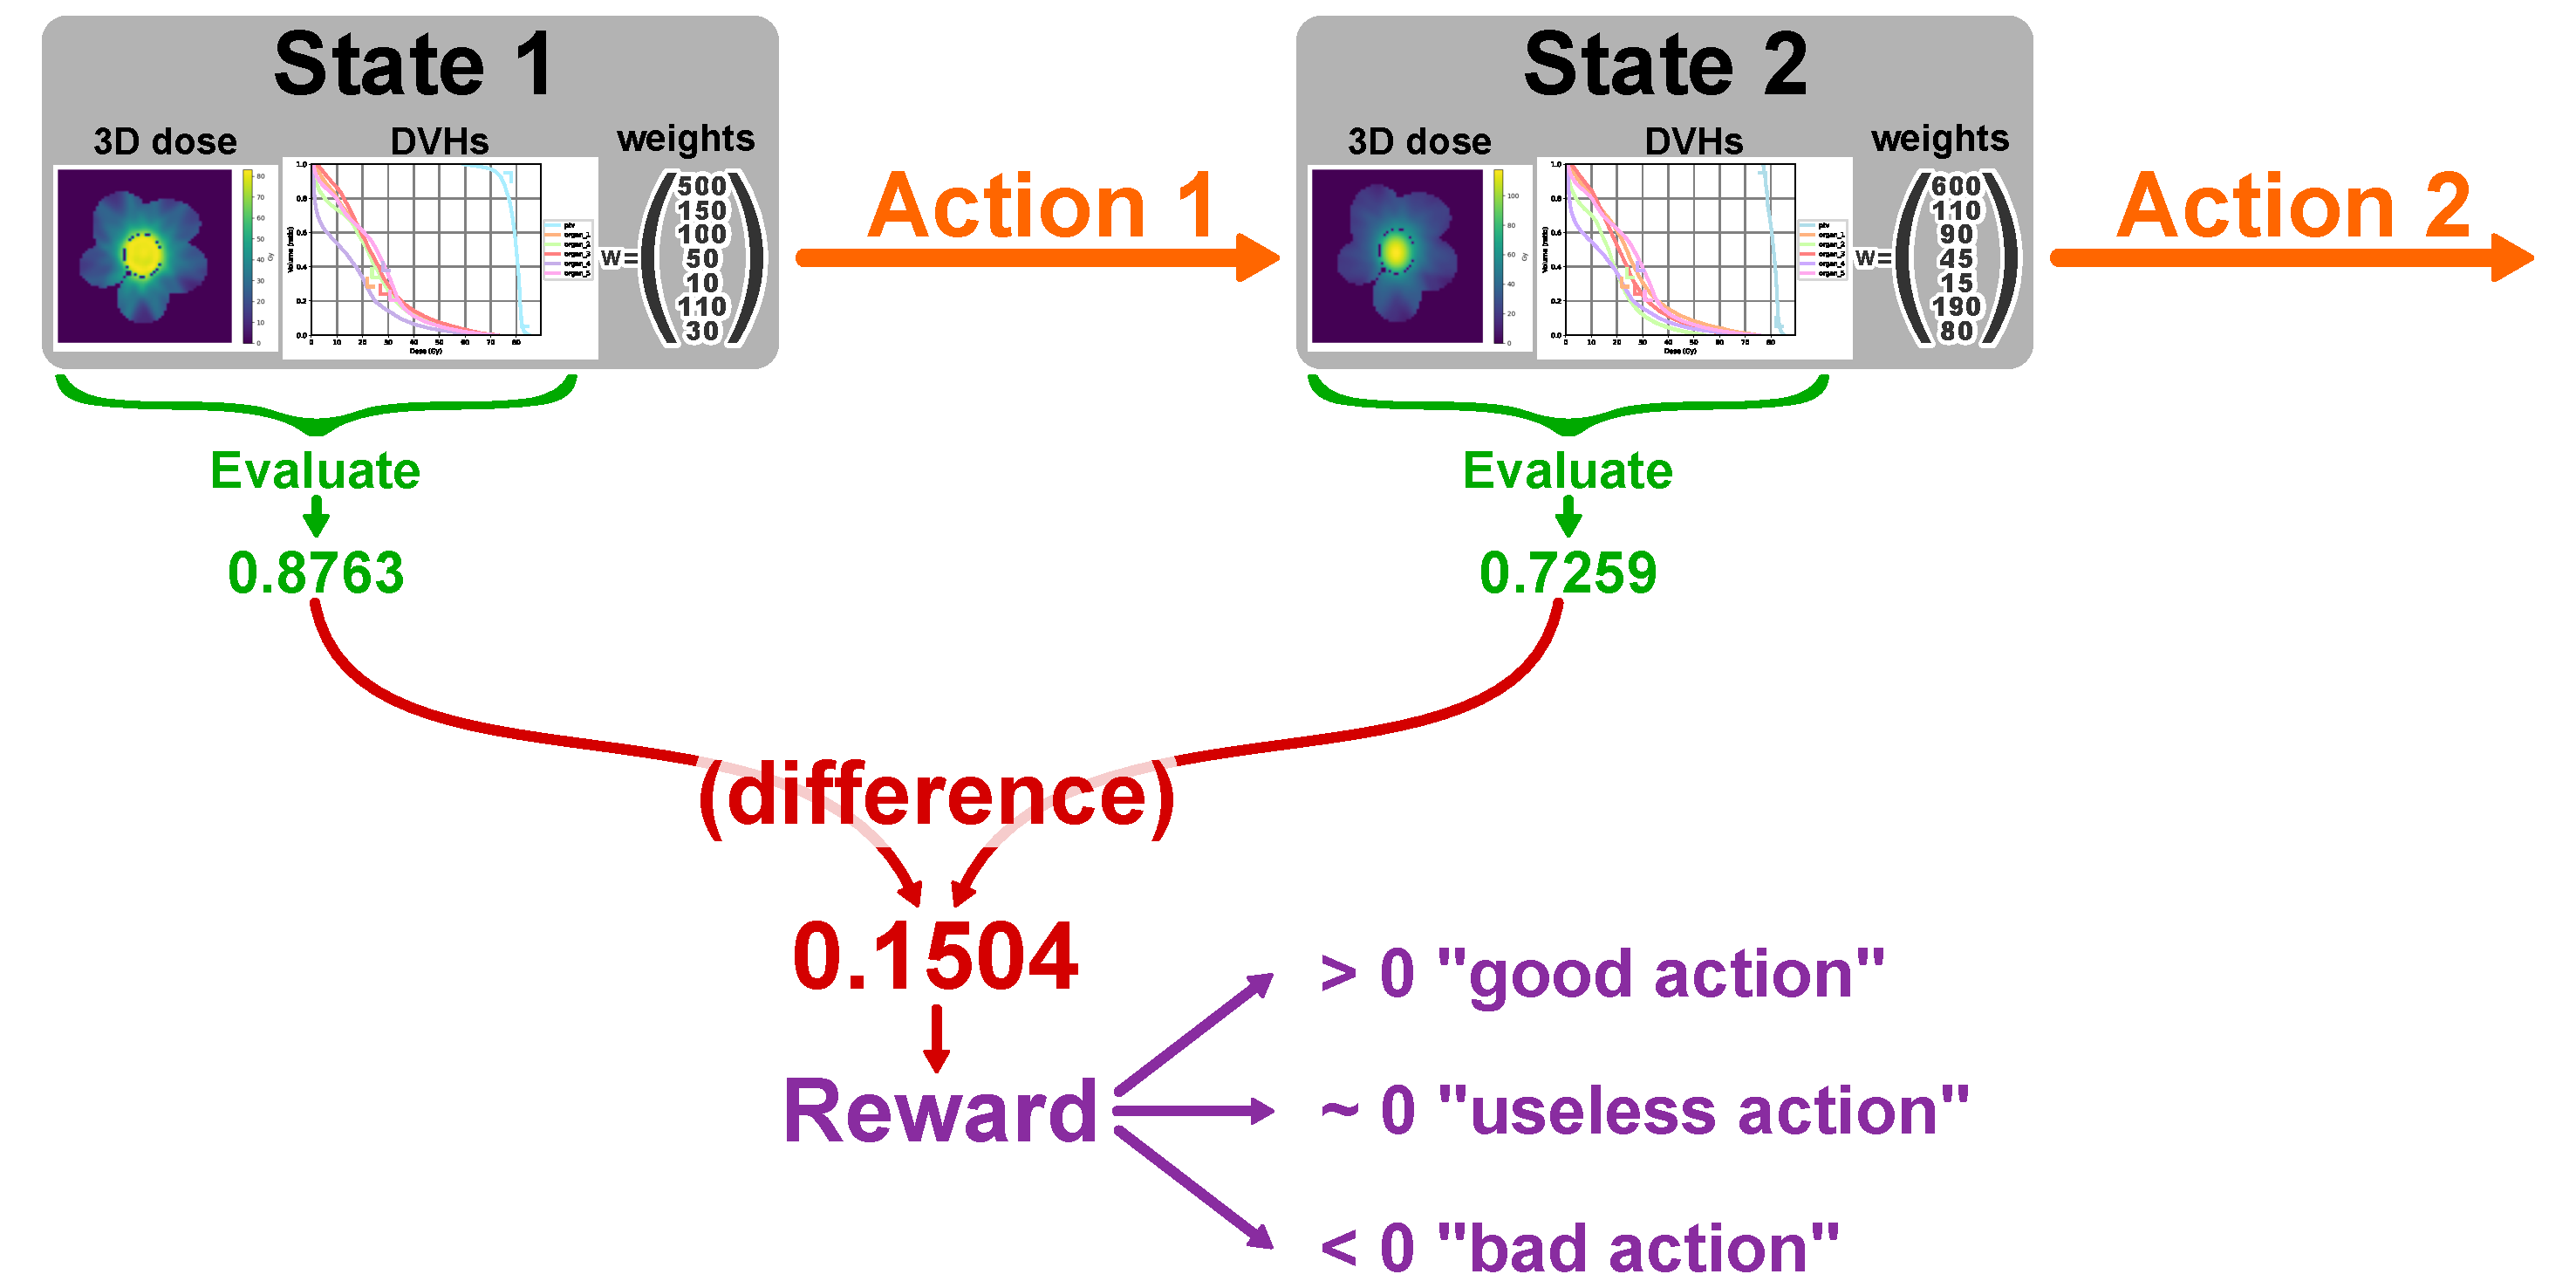
\includegraphics[width=0.8\textwidth]{reward.pdf}
	\caption{Classical reinforcement learning reward for automatic dosimetry.}
	\label{fig:reward_fig}
\end{figure*}

In classical RL, we want $V(S_t) = R_t + \gamma V(S_{t+1})$
(so the update is $V(S_t) \leftarrow (1-\alpha) V(S_t) + \alpha \left[ R_{t+1} + \gamma V(S_{t+1}) \right]$).
In the context of dose optimization, the reward $R_t$ is defined as $R_t = \mathcal{E}(S_{t+1}) - \mathcal{E}(S_t)$.
Where $\mathcal{E}$ is a function that evaluates the quality of a state (such that higher is better; if lower is better, then swap $s_t$ and $S_{t+1}$).

The evaluation $\mathcal{E}$ can be one or a mixture of the metrics mentioned in the introduction (Section \ref{metrics}) \cite{shen_hierarchical_2021} \cite{shen_intelligent_2019} \cite{moreau_reinforcement_2021}.
This setup may leverage knowledge about which actions to perform instead of guessing randomly as a meta-optimizer would do.
We can hope to gain some computation time.

However, this technique does not use past plans; it only needs the optimizer inputs (CT, structures contours).
We propose using the availability of past treatment plans to better catch the complexity of decisions made by dosimetrists and better match their expectations of a fully automatic treatment planning system.

As developed in previous work, we can derive a distance between dose plans [add citation].
If we consider the clinical dose of past cases (used for training) as the best achievable one, we can evaluate a dose plan by computing its distance from the clinical dose plan.

Let $D_t$ be the dose associated with $S_t$, and $D_C$ the clinical dose.
We then define $\mathcal{E}(S_t) = \mathcal{D}(D_t, D_C)$.
Since in that case, lower is better, we will define the reward as $$R_t = \mathcal{E}(S_t) - \mathcal{E}(S_{t+1}) = \mathcal{D}(D_t, D_C) - \mathcal{D}(D_{t+1}, D_C).$$
This reward can be interpreted as the "distance gained to the clinical dose".


\subsection{Reward-Free Reinforcement Learning}

Since the reward is based on an evaluation of the state, one may drop all the reward machinery and directly use the state evaluation.
This allows us to capture the signal better: it is not embedded in a reward system, and the network can learn faster.

The reason why the reward system is used in many games (such as go or chess) is that state evaluation is challenging, if not impossible; there is no function that, given the board, gives the quality of white/black's position.
A reward is only given at the end of a game, usually $+1$ for winning and $-1$ for losing.
The state's evaluation is deduced by the reinforcement learning agent while learning to maximize the reward.

However, in our dosimetrist case, we have precisely such an evaluation function.
Embedding this evaluation in a reward by defining the reward as the evaluation difference turns out to dilute the signal, and the agent learns slower.

By predicting the next state evaluation instead of using the Bellman optimality equation, we lose the ability to make short-term concessions in order to obtain large rewards later on.
In our case, making short-term concessions would mean that we trigger the weights in a way that the optimizer performs worse, but such that triggering a little more makes the optimizer perform better.
Given the problem we are solving (optimization of a radiotherapy dose), this is highly unlikely.

Because optimizers have the terrible habit of getting stuck in a local minimum, we can not use the last optimization result as a "warm start" after modifying optimization weights.
Hence, restarting optimization from zero is forced after every weight modification.

Given the statement of the optimization problem, and the fact that we can not use a warm start, making short-term compromises does not make much sense.
It is, therefore, safe to predict the next state evaluation directly, without the use of the Bellman optimality equation.

\subsection{Avoiding Over-fitting}
We use a dense neural network, taking the DVHs and the current normalized weight values as inputs.
Dense layers are very prone to overfitting.
In order to force the network to actually predict the following evaluation for each possible action, without over-fitting, we incorporated a bottleneck in the network.
Compressing the information stops the network from learning "by heart".
Networks with such architecture show significantly better results on validation.
%This comforted the idea that our network was learning from data without unthinkingly over-fitting.

\subsection{Avoiding Off-Distribution}
We generated a training set of over 125k actions (this took five days on an NVIDIA GeForce GTX 1080).
Despite this relatively large dataset, we have not explored exhaustively the state-actions space, and the network still gets off distribution.
This can easily be spotted when the predicted distance is negative; we choose to ignore those predictions.
In fact, we ignore all outlier predictions.
The justification is that our set of actions is limited, no action will suddenly drastically improve the plan.
It is the combination of several sequential actions that allows good plan optimization.
Therefore, while testing, we choose the action with the best prediction, while passing the outlier test just mentioned.

\section{Results}
In this section, we present the results obtained from our research.
Our primary objective was to mimic the dose with Reinforcement Learning (RL).

\subsection{Quantitative Results}
Our quantitative results indicate a significant improvement in dose mimicry using RL.
The statistical analysis showed a p-value less than 0.05, indicating that the results are statistically significant.
%The exact figures and graphs representing these results are presented in Figure X and Table Y.

\subsection{Qualitative Results}
Qualitatively, the RL model demonstrated superior performance in mimicking the dose.
The model managed to accurately predict the dose in various scenarios, showing its robustness and versatility.

\subsection{Comparison with Previous Work}
Compared to previous methods, our RL-based approach showed a marked improvement.
It outperformed traditional methods by Z\%, demonstrating the effectiveness of RL in this application.

\section{Discussion}
The results confirmed the effectiveness of reinforcement learning for mimicking the dose using DVH distance to derive the reward.
We aim to extend this work to real cases, with more constraints and complex decisions.

\section*{Appendix}
As this is very new and ongoing research, we generated synthetic phantom patients and associated trustable clinical doses.
In future work, we hope to apply this technique to real cases.

\subsection*{Synthetic phantom patients}
We generated 130 patients with oval axial section bodies.
We set the body density to water density.
We then added an ellipsoid PTV within the body, with a slightly different density (following $\mathcal{N}(1,0.05)$).
Likewise, we generate five organs gravitating around the PTV, aligned on the axial section.

\begin{figure*}
	\centering
	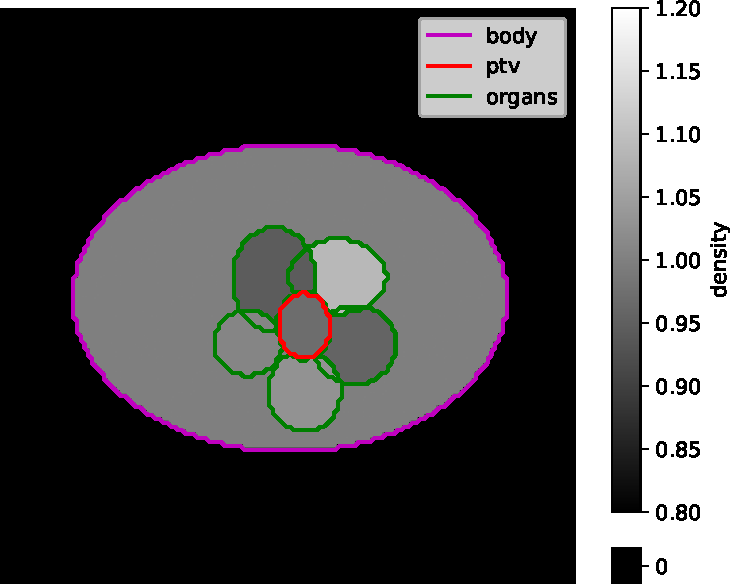
\includegraphics[width=0.7\textwidth]{main_slice-ct.pdf}
	\caption{first generated patient: Main axial slice (centre of the PTV) \textbf{CT}.\\ Structures are also contoured with legend.}
	\label{fig:main_slice-ct}
\end{figure*}

\subsection*{Clinical dose}
After generating the patient's CT and structures, we needed to create a reference dose that our agent should mimic.
We manually set weights and performed a standard optimization.

\begin{figure*}
	\centering
	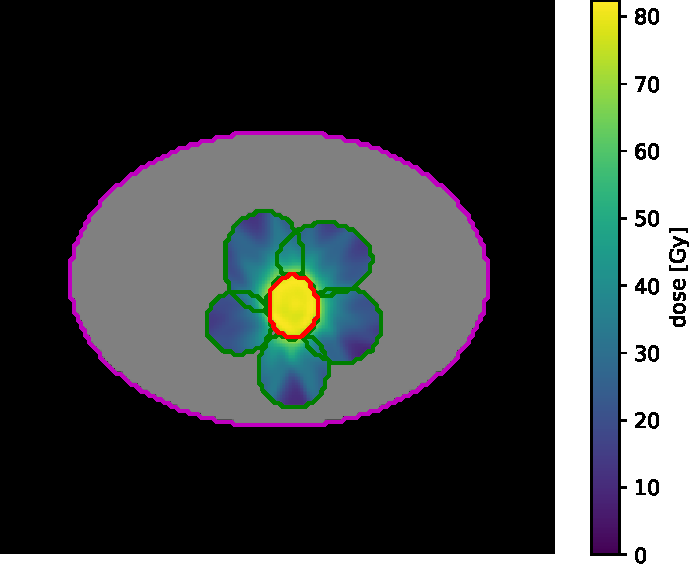
\includegraphics[width=0.7\textwidth]{main_slice-dose.pdf}
	\caption{First generated patient: main axial slice (centre of the PTV) of the \textbf{clinical dose}; structures are contoured as before.}
	\label{fig:main_slice-dose}
\end{figure*}
\begin{figure*}
	\centering
	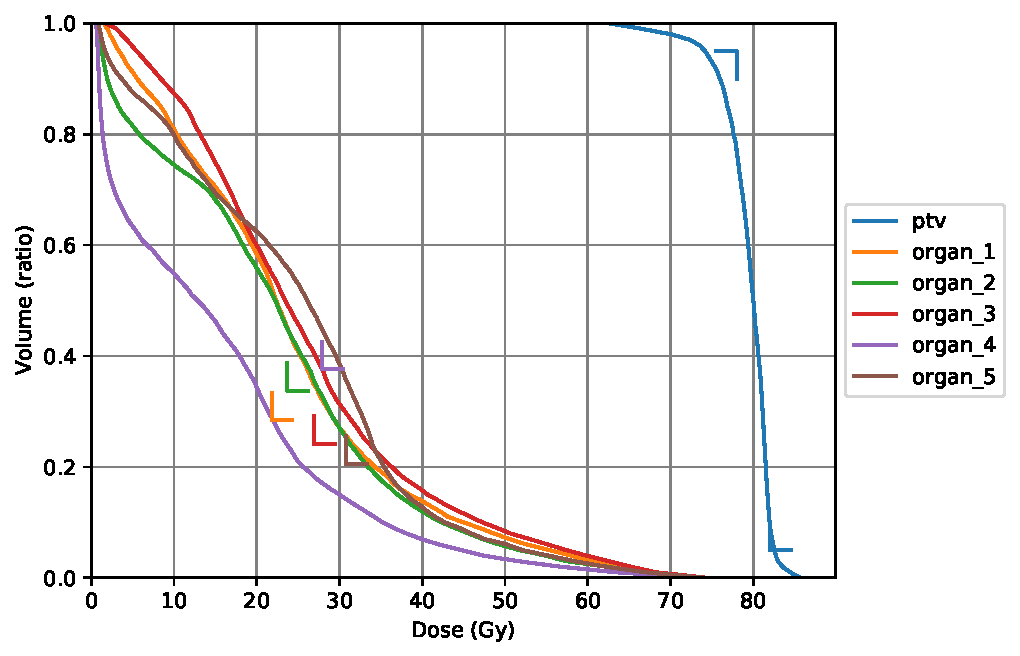
\includegraphics[width=0.9\textwidth]{dvh_example.pdf}
	\caption{First generated patient: clinical dose \textbf{DVH}.}
	\label{fig:clinical_dvh}
\end{figure*}

\subsection*{Optimization}
We optimize the plan using the LBFGS optimizer (shown to be the most appropriate in \cite{dubois_radiotherapy_2023}), with a learning rate of $0.03$.
Given the list of DVH constraints (e.g. for PTV, $D_{95}>80 \ Gy$), we use a linear penalization of the overdose.
Summing the multiplication of each cost term with the corresponding weight gives our objective function.
